\documentclass{article}
\usepackage{titlesec}
\usepackage[utf8]{inputenc}
\usepackage[a4paper, total={6in, 9in}]{geometry}
\usepackage{fancyhdr}
\usepackage{graphicx} % Add the graphicx package
\usepackage{lipsum} % For placeholder text
\usepackage{tikz}
\usepackage{cite}
\usepackage{bm}
\usepackage{acronym}
\usepackage{amsmath,amssymb,amsfonts}
\usepackage{algorithmic}
\usepackage{graphicx}
\usepackage{textcomp}
\usepackage{xcolor}
\usepackage[numbers]{natbib}
\bibliographystyle{ieeetrann}
\usepackage{multicol}
\usepackage{float}
\usepackage{circuitikz}
\usepackage{multirow}
\usepackage{url}


% Set up page headers and footers
\pagestyle{fancy}
\fancyhf{}
\rhead{Circuit Pirates}
\lhead{Three Channel Audio Mixer with Equalizers}
\cfoot{\thepage}

% Redefine the abstract environment to be single column
\renewenvironment{abstract}
{\par\noindent\textbf{\abstractname}\ \ignorespaces}{\par}

% Redefine section format
\titleformat{\section}
{\normalfont\Large\bfseries}{\thesection}{1em}{}

\begin{document}
	
	% Cover Page
	\begin{titlepage}
		
		\centering
		\vspace*{0.5cm}
		\includegraphics[width=5cm]{University_of_Moratuwa_logo.png} % Replace with the path to your university logo
		\par\vspace{0.02cm}
		{\fontfamily{lmss}
			{\Large Department of Electronic \& Telecommunication Engineering,\\
				University of Moratuwa, Sri Lanka.}}
		\par\vspace{2cm}
		{\LARGE\bfseries Three Channel Audio Mixer with Equalizers\par}
		\vspace{6cm}
		{\large Group Members:\par}
		\begin{tabular}{l l}
			& \\
	Member 1 230130E	&	Deshan W.U.\\
    Member 2 230138K	&	Dhananjaya K.T.G.T.N.\\
    Member 3 230155J	&	Dissanaka D.M.D.P.\\
    Member 4 230449N    &   Nuwanaka W.A.S.\\
		\end{tabular}\\
		\vspace{1.5cm}
		{Submitted in partial fulfillment of the requirements for the module\par}
		{EN 2091 Laboratory Practice and Projects\par}
	
		\vspace{1.0cm}
		{ Date: \today}
		\vfill
	\end{titlepage}
	
	\newpage
	
	\begin{abstract}\\
    This project presents a compact analog audio mixer featuring three independent input channels, each equipped with a dedicated three-band equalizer—Bass (20–250 Hz), Mid (250 Hz–4 kHz), and Treble (4–20 kHz). The system enables precise tonal shaping of each channel through variable gain control stages, allowing users to amplify or attenuate specific frequency ranges according to acoustic needs. Signal processing is implemented using low-noise operational amplifiers (NE5532 and TL072), while the TDA2030A provides robust output amplification. BC547 transistors are employed for pre amplification. The mixer’s compact PCB layout ensures efficient signal routing and minimal footprint, making it suitable for portable and space-constrained applications. This design demonstrates practical applications of analog circuit principles, including multi-band filter design, signal mixing, component-level optimization, and system integration for real-world audio enhancement.
\end{abstract}
	\section*{Abbreviations and Acronyms}
	\begin{acronym}
		\acro{OpAmp}{Operational Amplifier}
		\acro{PCB}{Printed Circuit board}
		\acro{THD}{Total Harmonic Distortion}
		\acro{JFET}{Junction Field Effect Transistor}
        \acro{SNR}{Signal to noise ratio}
	\end{acronym}
% 	\newpage
	
% \section*{Abbreviations and Acronyms}

% \begin{acronym}
% 	\acro{API}{Application Programming Interface}
% 	\acro{HTML}{Hypertext Markup Language}
% 	\acro{CSS}{Cascading Style Sheets}
% 	\acro{PDF}{Portable Document Format}
% \end{acronym}


	\newpage
	% Table of Contents
	\tableofcontents
	\newpage
	
	% Sections
	\section{Introduction and Functionality}
With the rapid growth of content creation among entry-level artists and the general public, the demand for compact, lightweight, and cost-effective audio mixers has increased significantly. Professional-grade sound mixers, although highly capable, are often expensive and bulky, making them unsuitable for beginners and small-scale applications.

To address this limitation, there is a growing need for portable and user-friendly audio mixing devices that offer essential audio processing features without excessive complexity. Audio mixers play a vital role in combining multiple audio sources and adjusting signal levels to achieve balanced and high-quality sound output.

The Three Channel Audio Mixer with Equalizers, developed by Circuit Pirates, is designed to fulfill this requirement. The system enables users to mix three independent audio inputs while providing equalization control to adjust low, mid, and high frequency components. This makes the mixer suitable for applications such as music recording, podcast production, live streaming, and educational audio experiments, where simplicity, affordability, and performance are equally important.
	
	
	\section{System Architecture}



\begin{figure}[htbp]
	\centering
	\includegraphics[width=1\textwidth]{sys_architecture.png}
	\caption{Example Figure.}
	\label{fig:Functional Block Diagram}
\end{figure}


\subsection{Pre Amplifier}
\subsubsection*{Mic Pre-amplifier}
For the mic pre-amplifier we used a cascaded transistor based amplifier in common emitter configuration with voltage divider bias.This ensured the thermal stability and the preferred gain.(gain ~160) Moderate input impedance and high output impedance was required by the mic input, this BJT configuration ensured these needs.
\subsubsection*{Instrument Pre-amplifier}
For the instrument pre amplifier high input impedance was required. So TL072 which is a JFET OPAMP is used since it requires very low input bias current.
Non inverting amplifier is used with few modifications added to filter DC signals and stabilize the output.

		\begin{figure}[H]
			\centering
			\includegraphics[width=\linewidth]{mic.png}
			\caption{MIC Pre-amp circuit schematic}
			\label{fig:right side view}
		\end{figure}
       

		\begin{figure}[H]
			\centering
			\includegraphics[width=\linewidth]{instrument.png}
			\caption{Instrument Pre-amp circuit schematic}
			\label{fig:Left side view}
		\end{figure}
	 
     
\newpage
\subsection{Equalizers}
Unity gain band-pass filters are implemented by cascading a second-order Sallen–Key low-pass filter with a second-order Sallen–Key high-pass filter. This configuration enables independent adjustment of the lower and upper cutoff frequencies, thereby providing flexible control over the passband characteristics.

%%%%%%%%%%%%%%%%%%%%%% High pass filter %%%%%%%%%%%%%%%%%%%%
\vspace{2em}
\noindent
\textbf{Second-order Sallen–Key low-pass filter}\cite{Filter_Design}
		
	\begin{multicols}{2}


		\begin{figure}[H]
        	\centering
        	\resizebox{0.5\textwidth}{!}{%
        		\begin{tikzpicture}
	% Paths, nodes and wires:
	\node[op amp, yscale=-1] at (8.19, 3.51){};
	\draw (-0, 4) to[european resistor, l={$R_1$}] (3.75, 4);
	\draw (3.75, 4) to[european resistor, l={$R_2$}] (7, 4);
	\draw (6.5, 5.75) to[capacitor, l={$C_2$}] (10.25, 5.75);
	\draw (6.5, 2.5) to[capacitor, l={$C_1$}] (6.5, -0.75);
	\node[eground] at (6.5, -0.75){};
	\node[ocirc](N1) at (0, 4){} node[anchor=east] at ([xshift=0.01cm]N1.text){$V_{in}$};
	\node[ocirc](N2) at (11.5, 3.5){} node[anchor=west] at (N2.text){$V_{out}$};
	\draw (3.75, 4) -- (3.75, 5.75) -- (6.5, 5.75);
	\draw (10.25, 5.76) -- (11, 5.76) -| (11, 3.51) |- (9.38, 3.52);
	\draw (6.5, 2.5) -| (6.5, 4);
	\draw (7, 3.02) |- (9.25, 2) -- (11, 2) -| (11, 3.51);
	\draw (11, 3.51) -| (11.5, 3.5);
	\node[circ] at (3.75, 4){};
	\node[circ] at (6.5, 4){};
	\node[circ] at (11, 3.52){};
\end{tikzpicture}
        	}
        	\caption{Sallen--Key low-pass filter}
        	\label{fig:SK_LPF}
        \end{figure}


        

  %%%%%%%%%%%%%%%%%%%%%%%% description %%%%%%%%%%%%%%%%%%%%%%%%%%      

        
		\begin{itemize}
			\item Cut-off frequency: $f_c = \frac{1}{2\pi\sqrt{{R_1R_2C_1C_2}}}$
			\item Dumping factor: $\zeta = \frac{R_1 + R_2}{2}\sqrt{\frac{C_1}{C_2R_1R_2}}$
			\item Filter quality: $Q = \frac{\zeta}{2}$
		
		\end{itemize}
\end{multicols}
    
\noindent
By selecting \( R_1 = R_2 = R \) and \( C_1 = C_2 = C \), the cutoff frequency simplifies to
\[
f_c = \frac{1}{2\pi RC}.
\]
Furthermore, under these conditions, the damping factor is \( \zeta = 1 \), corresponding to a critically damped response, and the quality factor is \( Q = 0.5 \).


   
%%%%%%%%%%%%%%%%%%%%%% High pass filter %%%%%%%%%%%%%%%%%%%%
\vspace{2em}
\noindent
\textbf{Second-order Sallen–Key high-pass filter}\cite{Filter_Design}
		\begin{multicols}{2}

	\begin{figure}[H]
        	\centering
        	\resizebox{0.5\textwidth}{!}{%
        		\begin{tikzpicture}
	% Paths, nodes and wires:
	\node[op amp, yscale=-1] at (8.19, 3.51){};
	\draw (6.5, 2.5) to[european resistor, l={$R_1$}] (6.5, -0.75);
	\draw (6.5, 5.75) to[european resistor, l={$R_2$}] (10.25, 5.75);
	\draw (0, 4) to[capacitor, l={$C_1$}] (3.75, 4);
	\node[eground] at (6.5, -0.75){};
	\node[ocirc](N1) at (0, 4){} node[anchor=east] at ([xshift=0.01cm]N1.text){$V_{in}$};
	\node[ocirc](N2) at (11.5, 3.5){} node[anchor=west] at (N2.text){$V_{out}$};
	\draw (3.75, 4) -- (3.75, 5.75) -- (6.5, 5.75);
	\draw (10.25, 5.75) -- (11, 5.75) -| (11, 3.5) |- (9.38, 3.51);
	\draw (6.5, 2.5) -| (6.5, 4);
	\draw (7, 3.02) |- (9.25, 2) -- (11, 2) -| (11, 3.51);
	\draw (11, 3.51) -| (11.5, 3.5);
	\node[circ] at (3.75, 4){};
	\node[circ] at (6.5, 4){};
	\node[circ] at (11, 3.52){};
	\draw (3.75, 4) to[capacitor, l={$C_2$}] (7, 4);
\end{tikzpicture}
        	}
        	\caption{Sallen--Key high-pass filter}
        	\label{fig:SK_LPF}
        \end{figure}
        

  %%%%%%%%%%%%%%%%%%%%%%%% description %%%%%%%%%%%%%%%%%%%%%%%%%%      

        
		\begin{itemize}
			\item Cut-off frequency: $f_c = \frac{1}{2\pi\sqrt{{R_1R_2C_1C_2}}}$
			\item Dumping factor: $\zeta = \frac{C_1 + C_2}{2}\sqrt{\frac{R_2}{R_1C_1C_2}}$
			\item Filter quality: $Q = \frac{\zeta}{2}$
		
		\end{itemize}
\end{multicols}


\noindent
Similar to the low-pass filter, by selecting \( R_1 = R_2 = R \) and \( C_1 = C_2 = C \), the cutoff frequency of the high-pass filter simplifies to
\[
f_c = \frac{1}{2\pi RC}.
\]
% \vspace{1em}  
Then again, under these conditions, the damping factor is \( \zeta = 1 \), corresponding to a critically damped response, and the quality factor is \( Q = 0.5 \).

\vspace{1.2em}  
\noindent
The above high-pass and low-pass filters are cascaded to form the unity gain band-pass filter.

\newpage
\begin{figure}[H]
		\centering
		% Resize to fit page width
		\resizebox{0.9\textwidth}{!}{%
			
			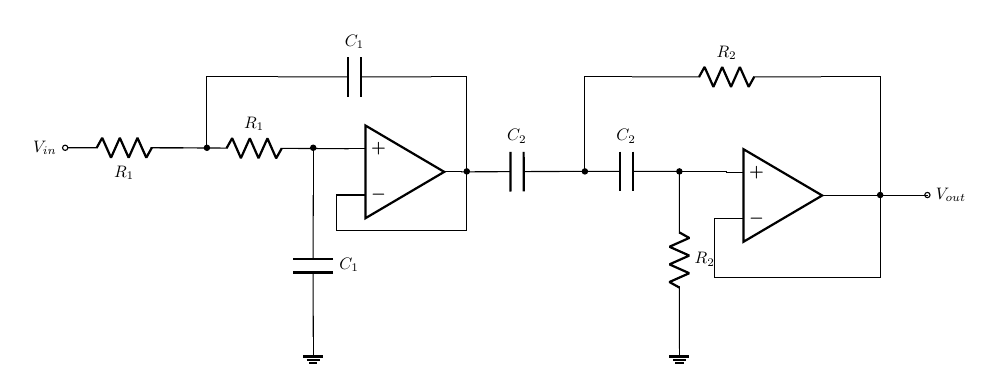
\begin{tikzpicture}[scale=0.6, transform shape]
				% Paths, nodes and wires:
				\node[op amp, yscale=-1] at (-14.81, 4.49){};
				\node[op amp, yscale=-1] at (-6.81, 3.99){};
				\draw (-20, 5) to[american resistor, l={$R_1$}] (-16, 4.98);
				\draw (-19.5, 5) to[american resistor, l={$R_1$}] (-22, 5);
				\draw (-10, 6.5) to[american resistor, l={$R_2$}] (-6, 6.5);
				\draw (-9, 4.5) to[american resistor, l={$R_2$}] (-9, 0.75);
				\draw (-17.5, 6.5) to[capacitor, l={$C_1$}] (-14.25, 6.5);
				\draw (-16.75, 4) to[capacitor, l={$C_1$}] (-16.75, 1);
				\draw (-13.62, 4.49) to[capacitor, l={$C_2$}] (-11.25, 4.5);
				\draw (-11.25, 4.5) to[capacitor, l={$C_2$}] (-9, 4.5);
				\draw (-9, 4.5) -- (-8, 4.5);
				\draw (-11.25, 4.5) -| (-11, 6.5) -- (-10, 6.5);
				\draw (-6, 6.5) -- (-4.75, 6.5) -| (-4.75, 4) |- (-5.62, 3.99);
				\draw (-8, 3.5) -- (-8.25, 3.5) -| (-8.25, 2.25) -| (-4.75, 3.99);
				\draw (-19, 5) -| (-19, 6.5) -- (-17.5, 6.5);
				\draw (-14.25, 6.5) -| (-13.5, 4.5);
				\draw (-16, 4) |- (-16.25, 4) -| (-16.25, 3.25) -- (-13.5, 3.25) -| (-13.5, 4.5);
				\draw (-16.75, 4) -| (-16.75, 5);
				\node[ground] at (-16.75, 1){};
				\node[ground] at (-9, 1){};
				\node[circ] at (-19, 5){};
				\node[circ] at (-16.75, 5){};
				\node[circ] at (-13.5, 4.5){};
				\node[circ] at (-11, 4.5){};
				\node[circ] at (-9, 4.5){};
				\node[circ] at (-4.75, 4){};
				\node[ocirc](N1) at (-22, 5){} node[anchor=east] at (N1.west){$V_{in}$};
				\node[ocirc](N2) at (-3.75, 4){} node[anchor=west] at (N2.east){$V_{out}$};
				\draw (-4.75, 3.99) -| (-3.75, 4);
			\end{tikzpicture}
		}
		\caption{Unity-Gain Sallen-Key Band-Pass Filter}
		\label{fig:Unity-Gain Sallen-Key Band-Pass Filter}
	\end{figure}

\subsubsection*{Calculated Theoretical Resistor \& Capacitor Values for Band-pass Filters}
    \begin{table}[h]
    \centering
    \renewcommand{\arraystretch}{1.3}
    \begin{tabular}{|c|cc|cc|}
    \hline
    \multirow{2}{*}{\textbf{Frequency band}} 
    & \multicolumn{2}{c|}{\textbf{Low pass filter}} 
    & \multicolumn{2}{c|}{\textbf{High pass filter}} \\
    \cline{2-5}
    & $R_1$ & $C_1$ & $R_2$ & $C_2$ \\
    \hline
    Low frequency band (50\,Hz -- 250\,Hz) 
    & $6.2\,\mathrm{k}\Omega$ & $100\,\mathrm{nF}$ 
    & $33\,\mathrm{k}\Omega$ & $100\,\mathrm{nF}$ \\
    \hline
    Mid frequency band (250\,Hz -- 4\,kHz) 
    & $3.9\,\mathrm{k}\Omega$ & $10\,\mathrm{nF}$ 
    & $6.2\,\mathrm{k}\Omega$ & $100\,\mathrm{nF}$ \\
    \hline
    High frequency band (4\,kHz -- 20\,kHz) 
    & $820\,\Omega$ & $10\,\mathrm{nF}$ 
    & $3.9\,\mathrm{k}\Omega$ & $10\,\mathrm{nF}$ \\
    \hline
    \end{tabular}
    \caption{Component values for band-pass filters}
    \end{table}

\noindent
However, slight variations were observed between the practical resistor and capacitor values and the theoretically calculated values, primarily due to component tolerances.

\subsection*{Gain Controller}
	\noindent
	\begin{minipage}{0.48\textwidth}
		\centering
		\begin{circuitikz}
			% Op-amp
			\node[op amp] (opamp) at (0.44, 4.49) {};
			
			% Input resistor
			\draw (-4.5, 5) to[american resistor, l={$R$}] (-0.38, 4.98);
			
			% Feedback resistor (variable)
			\draw (-0.75, 6.25) to[variable american resistor, l={$R_{v}$}] (2.25, 6.25);
			
			% Feedback wiring
			\draw (-0.75, 6.25) -- (-1, 6.25) -| (-1, 5);
			\draw (-0.75, 4) -- (-1, 4) -| (-1, 2.75);
			
			% Output connection
			\draw (1.63, 4.49) -| (2.5, 4.5) -- (2.5, 6.25) -- (2.25, 6.25);
			
			% Input/output nodes
			\node[ocirc](N1) at (-4.5, 5){} node[anchor=east] at (N1.west){$V_{in}$};
			\draw (2.5, 4.49) -| (2.75, 4.5);
			\node[ocirc](N2) at (2.75, 4.49){} node[anchor=west] at (N2.east){$V_{out}$};
			
			% Ground and connection dots
			\node[circ] at (-1, 5) {};
			\node[circ] at (2.5, 4.5) {};
			\node[ground] at (-1, 2.75) {};
		\end{circuitikz}
        
		\captionof{figure: }{Gain Controller}
		\label{fig:GainController}
	\end{minipage}%
	\hfill
	\begin{minipage}{0.48\textwidth}
		\[
		\frac{V_{in}-0}{R} = \frac{0 - V_{out}}{R_{v}}
		\]
		\[
		V_{out} =  \frac{R_{v}}{R}V_{in}
		\]
	\end{minipage}
	\newpage
\subsection{Power Amplifier Design}
The power amplifier circuit was taken from the datasheet of the TDA2030A IC by ST Microelectronics.\cite{TDA2030A_datasheet}
        \begin{figure}[H]
			\centering
			\includegraphics[width=0.6\linewidth]{power_amplifier.png}
			\caption{Power apmplifier circuit design.}
			\label{fig:pow}
		\end{figure}


\subsection{Power supply}
    12V dual supply was designed. Additionally coupling capacitors were added to remove the ripple.
     \begin{figure}[H]
			\centering
			\includegraphics[width=\linewidth]{Power supply.png}
			\caption{Power supply circuit design.}
			\label{fig:pow}
		\end{figure}
    
	
	\section{Component Selection}

  \begin{enumerate}

    % ============================
    % BC547B
    % ============================
    \item \textbf{BC547B NPN Transistor (Audio Applications) \cite{Fairchild-BC547}}
    \begin{itemize}
        \item \textbf{Low Noise BJT}: Suitable for small‑signal audio preamplifiers
        \item \textbf{Low Input Noise Current}: Ideal for microphone and sensor front‑ends
        \item \textbf{High Gain (h\textsubscript{FE})}: 200–450 typical for clean signal amplification
        \item \textbf{Low Distortion}: Works well in linear amplifier stages
        \item \textbf{Collector Current}: Up to 100\,mA for small audio drivers
        \item \textbf{Common Use}: Input stages, tone controls, preamp gain blocks
        
    \end{itemize}

    % ============================
    % NE5532
    % ============================
    \item \textbf{NE5532 Dual Low‑Noise Audio Operational Amplifier \cite{TI:NE5532}}
    \begin{itemize}
        \item \textbf{Ultra‑Low Noise}: 5\,nV/$\sqrt{\text{Hz}}$ for high‑fidelity audio
        \item \textbf{Low THD}: 0.0005\% typical for clean reproduction
        \item \textbf{High Slew Rate}: 9\,V/$\mu$s supports wide dynamic range
        \item \textbf{Wide Bandwidth}: 10\,MHz GBW for full audio spectrum accuracy
        \item \textbf{High Output Drive}: Can directly drive 600\,$\Omega$ loads
        \item \textbf{Common Use}: Headphone amps, mixers, equalizers, DAC/ADC buffers
    \end{itemize}

    % ============================
    % TL072
    % ============================
    \item \textbf{TL072 JFET‑Input Audio Operational Amplifier 
    \cite{TI:TL072}}
    \begin{itemize}
        \item \textbf{JFET Inputs}: Very high input impedance for guitar/piezo pickups
        \item \textbf{Low Noise}: 15\,nV/$\sqrt{\text{Hz}}$ suitable for musical instrument preamps
        \item \textbf{High Slew Rate}: 16\,V/$\mu$s for fast transient response
        \item \textbf{Low Distortion}: 0.01\% typical across audio band
        \item \textbf{Warm JFET Sound}: Preferred in analog synths and guitar pedals
        \item \textbf{Common Use}: Tone shaping, buffers, active filters, effects pedals
    \end{itemize}

    % ============================
    % TDA2030A
    % ============================
    \item \textbf{TDA2030A Class‑AB Audio Power Amplifier \cite{TDA2030A_datasheet}}
    \begin{itemize}
        \item \textbf{Output Power}: Up to 20\,W for compact speaker systems
        \item \textbf{Low THD}: Very low harmonic and crossover distortion
        \item \textbf{High Output Current}: Drives 4\,$\Omega$ and 8\,$\Omega$ speakers
        \item \textbf{Wide Frequency Response}: Suitable for full‑range audio
        \item \textbf{Stable Class‑AB Operation}: Smooth, warm analog sound
        \item \textbf{Common Use}: Active speakers, subwoofer modules, DIY amplifiers
    \end{itemize}

\end{enumerate}
	
	\section{PCB Design}
   We implemented a modular approach where we used 3 separate PCB s for the channels and a single PCB to combine and power amplify the signal. The power supply was made as a separate PCB to reduce the power supply noise interference with audio.

\subsection*{Signal Integrity and Noise Reduction}
The PCB layout was created with a focus on reducing noise and maintaining signal integrity. Sensitive input paths were routed away from switching or high-current nodes, and low-level audio traces were kept as brief as possible to minimize interference. 

\subsection*{Grounding Strategy}
To avoid ground loops and get a clear audio performance, a star-ground strategy was used. Analog grounds for each channel were separated throughout the board and joined only at a single point. 

\subsection*{Power Supply and Decoupling}
Each channel was provided with local decoupling capacitors, combining 100\,nF ceramic capacitors for high-frequency filtering and 10\,µF electrolytic capacitors for reducing low-frequency voltage ripple. The power supply section was \textbf{physically isolated} from the audio signal paths, ensuring clean ±12\,V rails for the mixer.

\subsection*{Component Placement and Routing}
In order to support both mechanical usability and electrical performance, component placement was optimised. To reduce loop area, op-amps were positioned near their corresponding feedback networks. Potentiometers were positioned for front-panel mounting, and input connectors were placed close to the preamplifier stage to minimise trace length. Thinner traces were used for low-level audio signals, and wider traces were used for power and output paths.

\subsection*{Thermal and Mechanical Considerations}
Thermal considerations were taken into consideration even though the mixer mostly uses low-power analogue components. To enable heat dissipation, components like output drivers and voltage regulators were positioned close to the board's edges. 
We used a cooling fan to maximize the air flow and hence effectively cool down the power amplifier and voltage regulator ICs.


\begin{multicols}{2}
		\begin{figure}[H]
			\centering
			\includegraphics[width=0.6\linewidth]{channels.png}
			\caption{Routing diagram of channel equalizer, preamplifier PCB.}
			\label{fig:channels2d}
		\end{figure}
		\begin{figure}[H]
			\centering
			\includegraphics[width=0.6\linewidth]{channels_PCB.png}
			\caption{3D diagram of channel equalizer, pre amplifier PCB.}
			\label{fig:channels3d}
		\end{figure}
\end{multicols}
        \begin{multicols}{2}
		\begin{figure}[H]
			\centering
			\includegraphics[width=0.6\linewidth]{mixer.png}
			\caption{Routing diagram of channel mixer, power amplifier PCB.}
			\label{fig:mixer}
		\end{figure}
		\begin{figure}[H]
			\centering
			\includegraphics[width=0.6\linewidth]{mixer_PCB.png}
			\caption{3D diagram of channel equalizer, preamplifier mixer, power amplifier PCB.}
			\label{fig:display}
		\end{figure}
        \end{multicols}
        
        \begin{multicols}{2}
            
		\begin{figure}[H]
			\centering
			\includegraphics[width=0.5\linewidth]{power.png}
			\caption{Routing diagram of channel power supply PCB.}
			\label{fig:pow}
		\end{figure}
        \begin{figure}[H]
			\centering
			\includegraphics[width=0.5\linewidth]{power_PCB.png}
			\caption{3D diagram of channel power supply PCB.}
			\label{fig:pow}
		\end{figure}
        \end{multicols}
        


    \newpage
	\section{Enclosure Design}
    The enclosure was designed to protect the electronic components from mechanical damage and to electrically isolate them from the user. The overall dimensions of the enclosure are 17.5 cm in width and 22.5 cm in length. The height of the shorter side is 3.6 cm, while the taller side has a height of 7.0 cm. A wall thickness of 3 mm was selected to increase the mechanical strength and rigidity of the enclosure.

% \vspace{0.5em} 
% \noindent
A space with dimensions of 7 cm × 17.5 cm and a constant height of 7.0 cm was reserved for placing the transformer and the cooling fan. All PCBs, except the power supply PCB, were mounted vertically inside the enclosure and secured using screws.

% \vspace{0.5em} 
% \noindent
Ventilation holes were provided on both the left and right sides, as well as on the rear side of the enclosure, to facilitate adequate airflow and heat dissipation. Polylactic Acid (PLA) was selected as the material for 3D printing.

% \vspace{0.5em} 
% \noindent
To reduce the overall 3D printing cost, two bottom support structures were printed as separate components and subsequently attached to the enclosure during assembly.

\vspace{2.5em} 
	\begin{multicols}{2}
		\begin{figure}[H]
			\centering
			\includegraphics[width=\linewidth]{front.png}
			\caption{Enclosure front view}
			\label{fig:Enclosure front view}
		\end{figure}
		\begin{figure}[H]
			\centering
			\includegraphics[width=\linewidth]{back.png}
			\caption{Back view}
			\label{fig:back view}
		\end{figure}
    \end{multicols}

    \vspace{2em} 
    \begin{multicols}{2}
		\begin{figure}[H]
			\centering
			\includegraphics[width=\linewidth]{right side.png}
			\caption{Right side view}
			\label{fig:right side view}
		\end{figure}
		\begin{figure}[H]
			\centering
			\includegraphics[width=\linewidth]{left side.png}
			\caption{Left side view}
			\label{fig:Left side view}
		\end{figure}
	 \end{multicols}
     
\vspace{2em} 
    \begin{multicols}{2}
		\begin{figure}[H]
			\centering
			\includegraphics[width=\linewidth]{main part.png}
			\caption{Inside view}
			\label{fig:Inside view}
		\end{figure}
		\begin{figure}[H]
			\centering
			\includegraphics[width=\linewidth]{lid.png}
			\caption{Lid}
			\label{fig:Lid}
		\end{figure}
	 \end{multicols}

       \begin{figure}[H]
        \centering
        \includegraphics[width=0.5\linewidth]{final product.jpg}
        \caption{Final product}
        \label{fig:placeholder}
    \end{figure}
     
	\newpage
	\section{Software Simulation and Hardware Testing}
    \subsection{Software simulation}
    Software simulation was done with LTspice software. Pre amplifier, filter circuits were tested individually and combined later.

    \begin{multicols}{2}
		\begin{figure}[H]
			\centering
			\includegraphics[width=\linewidth]{preamp_lt.png}
			\caption{Pre amplifier circuit}
			\label{fig:Pre amp testing.}
		\end{figure}
		\begin{figure}[H]
			\centering
			\includegraphics[width=\linewidth]{preamp_graph.png}
			\caption{LT spice simulation output.}
			\label{fig:LTspice simulation output}
		\end{figure}
    \end{multicols}

    
    \begin{multicols}{2}
		\begin{figure}[H]
			\centering
			\includegraphics[width=\linewidth]{instrument amp_lt.png}
			\caption{Pre amplifier circuit for instruments.}
			\label{fig:Pre amp testing.}
		\end{figure}
		\begin{figure}[H]
			\centering
			\includegraphics[width=\linewidth]{instrument_preampgraph.png}
			\caption{LT spice simulation output.}
			\label{fig:LTspice simulation output}
		\end{figure}
    \end{multicols}

    
    \begin{multicols}{2}
		\begin{figure}[H]
			\centering
			\includegraphics[width=\linewidth]{equalizer_testing.jpg}
			\caption{Equalizer LTspice simulation}
			\label{fig:Pre amp testing.}
		\end{figure}
		\begin{figure}[H]
			\centering
			\includegraphics[width=\linewidth]{equalizer_output.png}
			\caption{LT spice simulation frequency response for each frequency band.}
			\label{fig:LTspice simulation output}
		\end{figure}
    \end{multicols}
    
     \begin{figure}[H]
        \centering
        \includegraphics[width=0.8\linewidth]{equalizer_combined_graph.png}
        \caption{Equalizer Frequency response.}
        \label{fig:placeholder}
    \end{figure}
    
    
    \subsection{Hardware Testing}
    Hardware testing was carried out in two stages, first we implemented the circuits on breadboards and validated the design. 
    Second testing was done to ensure the PCB implementation is error free.
      \begin{figure}[H]
        \centering
        \includegraphics[width=0.9\linewidth]{hardware testing.jpg}
        \caption{Breadboard testing.}
        \label{fig:placeholder}
    \end{figure}

    
	\newpage
	\section{Conclusion \& Future Works}

    \subsection*{Conclusion}


    In this project, a 3-Channel Audio Mixer with a 3-Band Equalizer was successfully designed and implemented. The system allows independent control of low, mid, and high frequency bands for each input channel, providing flexibility in audio mixing and tone shaping. By using operational amplifiers, active RC filter networks, and proper buffering techniques, the mixer achieves stable operation with minimal distortion and acceptable noise performance.

    The mixer effectively combines multiple audio inputs into a single output while maintaining signal integrity. The practical implementation validated the theoretical design concepts studied in analog electronics, such as filter design, gain control, and signal summing. Testing results confirmed that the equalizer provides noticeable frequency adjustment and the overall system performs reliably for basic audio applications such as small audio setups, educational demonstrations, and laboratory use.

    This project enhanced our understanding of analog audio signal processing, circuit debugging, PCB layout considerations, and real-world implementation challenges.




    \subsection*{Future Work}
    


    Although the current design meets the project objectives, several improvements can be considered for future development:


    Class-D Power Amplifier Integration: The current system uses a Class-AB power amplifier, which provides good audio quality but has relatively lower efficiency and higher power dissipation. In future versions, a Class-D power amplifier can be implemented to significantly improve power efficiency, reduce heat generation, and enable compact and portable designs.
    Additional Channels: Expanding the design to support more input channels for advanced mixing applications.
    Balanced Inputs and Outputs: Implementing balanced XLR or TRS connectors to reduce noise and interference in professional audio environments.
    Power Supply Enhancement: Designing a regulated and isolated power supply to further reduce hum and noise.
    User Interface Improvements: Adding LED level indicators or VU meters to visually monitor signal levels.
    Enclosure Optimization: Improving mechanical design for better portability, durability, and thermal management.
    Bluetooth or USB Audio Support: Adding wireless or USB audio interfaces for modern connectivity.
    With these enhancements, the audio mixer can be transformed into a more versatile and professional-grade audio processing system suitable for wider real-world applications.
	\newpage
	\section{Contribution of Group Members}
	\begin{tabular}{|l|p{10cm}|}
\hline
\textbf{Student’s Name (Index No.)} & \textbf{Contribution} \\ \hline

K.T.G.T.N. Dhananjaya (230138K) & Circuit design, Circuit simulation, Enclosure design, Filter calculations \\ \hline
W.U. Deshan (230130E) & Breadboard implementation, Circuit design, Testing, Soldering, Assembling \\ \hline
D.M.D.P. Dissanayaka (230155J) & PCB design, Testing, debugging, Circuit design, Breadboard implementation \\ \hline
W.A.S. Nuwanaka (230449N) & Breadboard implementation, Testing, Soldering, Assembling \\ \hline
\end{tabular}
	
	\section*{Acknowledgment}

    We would like to express our sincere gratitude to all those who supported and guided us throughout the completion of this group project. We are deeply thankful to \textbf{Dr. Sampath Perera} for his valuable insights, encouragement, and continuous guidance, which greatly contributed to the quality of our work. We also extend our appreciation to \textbf{Ms. Sanjana Kapukotuwa} for the constructive feedback, technical assistance, and willingness to share their expertise whenever needed. Finally, we wish to thank the lab technicians for their support, service, and cooperation during the various stages of this project. Their collective contributions have been instrumental in the successful completion of our work.

    
\bibliography{ref}
\begin{thebibliography}{1}
		\bibitem{TIMixer_Design}
		Texas Instruments, \emph{Designing professional audio mixers for every scenario}, Rev. 8, Advanced Analog Products, SLOD006B, 2018. [Online]. Available: \url{https://www.ti.com/lit/wp/spry322/spry322.pdf?ts=1765656390235}

        
        
        \bibitem{TI:TL072}
		Texas Instruments,TL072 — Dual, 30‑V, 3‑MHz, low‑noise JFET‑input operational amplifier,”  
TI product page (Datasheet TL07xx family), [Online]. Available: \url{https://www.ti.com/lit/ds/symlink/tl072.pdf}  

		\bibitem{TI:NE5532}
		Texas Instruments, “NE5532 — Dual, 30-V, 10-MHz, low-noise operational amplifier for audio applications,”  
		TI product page (Datasheet Rev. J), Jan. 27, 2015.  
		[Online]. Available: \url{https://www.ti.com/product/NE5532}  
        
		\bibitem{Fairchild-BC547}
		“BC547 — NPN, low‑noise general‑purpose transistor,”  
ON Semiconductor product page (Datasheet BC546/BC547/BC548 series), [Online].  
Available: \url{https://cdn.sparkfun.com/assets/d/5/e/5/d/BC547.pdf}

		\bibitem{TDA2030A_datasheet}
    “TDA2030A — 18‑W, class‑AB audio power amplifier,”  
    STMicroelectronics product page (Datasheet Rev. 3), [Online].   Available:
\url{https://mm.digikey.com/Volume0/opasdata/d220001/medias/docus/1/TDA2030A.pdf}
		
		
        \bibitem{Filter_Design}
        S. Winder, "Analog and Digital Filter Design", \emph{2nd ed. Oxford, U.K.: Newnes, 2002.}
		Available: \url{https://www.sciencedirect.com/book/monograph/9780750675475/analog-and-digital-filter-design}
	
	\end{thebibliography}

\bibliographystyle{IEEEbib}
%\section{Appendix}

\title{Schematic diagrams.}	


\end{document}
